\documentclass[10pt,conference]{IEEEtran}
\usepackage{amsmath,amssymb,stmaryrd}
\usepackage{graphicx}
\usepackage{booktabs}
\usepackage{array}
\usepackage{adjustbox}
\usepackage{xcolor}
\usepackage{url}
\usepackage{listings}
\usepackage{algorithm}
\usepackage[noend]{algpseudocode}
\providecommand{\ket}[1]{\lvert #1\rangle}
\newcommand{\Bw}{B_{\mathrm{QDG}}}
\newcommand{\Fw}{F_{\mathrm{QDG}}}
\newtheorem{definition}{Definition}
\newtheorem{theorem}{Theorem}
\newtheorem{proposition}{Proposition}
% Generated by experiments/icpc/make_numbers.py from committed results. Do not edit by hand.

\newcommand{\numNPairs}{784}  % results/icpc/rq1/records.csv
\newcommand{\numNCircuits}{158}  % results/icpc/rq1/records.csv
\newcommand{\numRqOneDuUnsound}{216}  % results/icpc/rq1/records.csv
\newcommand{\numRqOneDuUnsoundPct}{27.6\%}  % results/icpc/rq1/records.csv
\newcommand{\numRqOneDuRecall}{0.718}  % results/icpc/rq1/records.csv
\newcommand{\numRqOneDuPrecision}{0.970}  % results/icpc/rq1/records.csv
\newcommand{\numRqOneDuSize}{51.2\%}  % results/icpc/rq1/records.csv
\newcommand{\numRqOneLcUnsound}{0}  % results/icpc/rq1/records.csv
\newcommand{\numRqOneLcUnsoundPct}{0.0\%}  % results/icpc/rq1/records.csv
\newcommand{\numRqOneLcRecall}{1.000}  % results/icpc/rq1/records.csv
\newcommand{\numRqOneLcPrecision}{0.923}  % results/icpc/rq1/records.csv
\newcommand{\numRqOneLcSize}{70.4\%}  % results/icpc/rq1/records.csv
\newcommand{\numRqOneYzUnsound}{0}  % results/icpc/rq1/records.csv
\newcommand{\numRqOneYzUnsoundPct}{0.0\%}  % results/icpc/rq1/records.csv
\newcommand{\numRqOneYzRecall}{1.000}  % results/icpc/rq1/records.csv
\newcommand{\numRqOneYzPrecision}{0.835}  % results/icpc/rq1/records.csv
\newcommand{\numRqOneYzSize}{78.6\%}  % results/icpc/rq1/records.csv
\newcommand{\numRqOneQUnsound}{0}  % results/icpc/rq1/records.csv
\newcommand{\numRqOneQUnsoundPct}{0.0\%}  % results/icpc/rq1/records.csv
\newcommand{\numRqOneQRecall}{0.807}  % results/icpc/rq1/records.csv
\newcommand{\numRqOneQPrecision}{0.972}  % results/icpc/rq1/records.csv
\newcommand{\numRqOneQSize}{54.0\%}  % results/icpc/rq1/records.csv
\newcommand{\numRqOneFourEdgeUnfixedUnsound}{5}  % results/icpc/rq1/records.csv
\newcommand{\numRqOneFourEdgeUnfixedUnsoundPct}{0.6\%}  % results/icpc/rq1/records.csv
\newcommand{\numRqOneFourEdgeUnfixedRecall}{0.994}  % results/icpc/rq1/records.csv
\newcommand{\numRqOneFourEdgeUnfixedPrecision}{0.864}  % results/icpc/rq1/records.csv
\newcommand{\numRqOneFourEdgeUnfixedSize}{75.0\%}  % results/icpc/rq1/records.csv
\newcommand{\numRqOneFourEdgeFixedUnsound}{0}  % results/icpc/rq1/records.csv
\newcommand{\numRqOneFourEdgeFixedUnsoundPct}{0.0\%}  % results/icpc/rq1/records.csv
\newcommand{\numRqOneFourEdgeFixedRecall}{1.000}  % results/icpc/rq1/records.csv
\newcommand{\numRqOneFourEdgeFixedPrecision}{0.864}  % results/icpc/rq1/records.csv
\newcommand{\numRqOneFourEdgeFixedSize}{75.2\%}  % results/icpc/rq1/records.csv
\newcommand{\numRqOneDuMissKickback}{1{,}737}  % results/icpc/rq1/misses.csv
\newcommand{\numRqOneDuMissSameWire}{835}  % results/icpc/rq1/misses.csv
\newcommand{\numRqOneDuMissWrittenOperand}{654}  % results/icpc/rq1/misses.csv
\newcommand{\numRqOneDuMissFeedback}{134}  % results/icpc/rq1/misses.csv
\newcommand{\numRqOneQRemoved}{2{,}847}  % results/icpc/rq1/pairs.csv
\newcommand{\numRqOneQRemovedNonInfluencing}{669}  % results/icpc/rq1/pairs.csv
\newcommand{\numRqOneQRemovedContributing}{1{,}618}  % results/icpc/rq1/pairs.csv
\newcommand{\numRqOneQPrunedPairs}{477}  % results/icpc/rq1/pairs.csv
\newcommand{\numLcqApplicable}{732}  % results/icpc/rq1_lcq_remap/records.csv
\newcommand{\numLcqNotApplicable}{52}  % results/icpc/rq1_lcq_remap/records.csv
\newcommand{\numLcqNaMeasurements}{42}  % results/icpc/rq1_lcq_remap/records.csv
\newcommand{\numLcqUnsound}{0}  % results/icpc/rq1_lcq_remap/records.csv
\newcommand{\numLcqSmallerThanLc}{243}  % results/icpc/rq1_lcq_remap/records.csv
\newcommand{\numLcqRecall}{0.93}  % results/icpc/rq1_lcq_remap/records.csv
\newcommand{\numQVsLcqReduction}{12.3\%}  % results/icpc/rq1_lcq_remap/records.csv
\newcommand{\numQVsLcqReductionPooled}{10.8\%}  % results/icpc/rq1_lcq_remap/records.csv
\newcommand{\numQLargerThanLcq}{72}  % results/icpc/rq1_lcq_remap/records.csv
\newcommand{\numHOnePHolm}{\ensuremath{p < 10^{-10}}}  % results/icpc/confirmatory/summary.json
\newcommand{\numHTwoDiff}{16.3}  % results/icpc/confirmatory/summary.json
\newcommand{\numHTwoCILow}{15.1}  % results/icpc/confirmatory/summary.json
\newcommand{\numHTwoCIHigh}{17.7}  % results/icpc/confirmatory/summary.json
\newcommand{\numHTwoRelative}{23.2\%}  % results/icpc/confirmatory/summary.json
\newcommand{\numHTwoSmaller}{477}  % results/icpc/confirmatory/summary.json
\newcommand{\numHTwoPHolm}{\ensuremath{p < 10^{-10}}}  % results/icpc/confirmatory/summary.json
\newcommand{\numHTwoR}{1.00}  % results/icpc/confirmatory/summary.json
\newcommand{\numHThreeRate}{55.4\%}  % results/icpc/confirmatory/summary.json
\newcommand{\numHThreeCILow}{51.9\%}  % results/icpc/confirmatory/summary.json
\newcommand{\numHThreeCIHigh}{58.8\%}  % results/icpc/confirmatory/summary.json
\newcommand{\numHThreePrunedRate}{26.6\%}  % results/icpc/confirmatory/summary.json
\newcommand{\numHThreePrunedRobust}{127}  % results/icpc/confirmatory/summary.json
\newcommand{\numHThreePrunedN}{477}  % results/icpc/confirmatory/summary.json
\newcommand{\numHFourContainQ}{82.2\%}  % results/icpc/confirmatory/summary.json
\newcommand{\numHFourContainLc}{95.7\%}  % results/icpc/confirmatory/summary.json
\newcommand{\numHFourDiff}{\ensuremath{-}13.5}  % results/icpc/confirmatory/summary.json
\newcommand{\numHFourCILow}{\ensuremath{-}14.4}  % results/icpc/confirmatory/summary.json
\newcommand{\numHFourCIHigh}{\ensuremath{-}12.6}  % results/icpc/confirmatory/summary.json
\newcommand{\numHFiveSizeDiff}{2.9}  % results/icpc/confirmatory/summary.json
\newcommand{\numHFiveExamDiff}{\ensuremath{-}0.061}  % results/icpc/confirmatory/summary.json
\newcommand{\numRobQPrunedBasis}{65.8\%}  % results/icpc/rq2_robustness/pairs.csv
\newcommand{\numRobLcBasis}{100.0\%}  % results/icpc/rq2_robustness/pairs.csv
\newcommand{\numRobQPrunedHaar}{26.6\%}  % results/icpc/rq2_robustness/pairs.csv
\newcommand{\numRobLcHaar}{100.0\%}  % results/icpc/rq2_robustness/pairs.csv
\newcommand{\numRobQPrunedParam}{78.1\%}  % results/icpc/rq2_robustness/pairs.csv
\newcommand{\numRobLcParam}{100.0\%}  % results/icpc/rq2_robustness/pairs.csv
\newcommand{\numRobLcqBasisRobust}{732}  % results/icpc/rq2_robustness_lcq/pairs.csv
\newcommand{\numRobLcqBasisN}{732}  % results/icpc/rq2_robustness_lcq/pairs.csv
\newcommand{\numRobLcqHaarRobust}{732}  % results/icpc/rq2_robustness_lcq/pairs.csv
\newcommand{\numRobLcqHaarN}{732}  % results/icpc/rq2_robustness_lcq/pairs.csv
\newcommand{\numRobLcqParamRobust}{171}  % results/icpc/rq2_robustness_lcq/pairs.csv
\newcommand{\numRobLcqParamN}{175}  % results/icpc/rq2_robustness_lcq/pairs.csv
\newcommand{\numAblUnfixedFull}{0.5\%}  % results/rq4_ablation/TAB_ablation_rerun.csv
\newcommand{\numAblUnfixedNoED}{54.0\%}  % results/rq4_ablation/TAB_ablation_rerun.csv
\newcommand{\numAblUnfixedNoMD}{13.4\%}  % results/rq4_ablation/TAB_ablation_rerun.csv
\newcommand{\numAblUnfixedNoUED}{13.3\%}  % results/rq4_ablation/TAB_ablation_rerun.csv
\newcommand{\numAblUnfixedNoCD}{4.8\%}  % results/rq4_ablation/TAB_ablation_rerun.csv
\newcommand{\numAblFixedFull}{0.0\%}  % results/icpc/ablation_fixed/TAB_ablation_rerun.csv
\newcommand{\numAblFixedNoED}{63.9\%}  % results/icpc/ablation_fixed/TAB_ablation_rerun.csv
\newcommand{\numAblFixedNoMD}{13.0\%}  % results/icpc/ablation_fixed/TAB_ablation_rerun.csv
\newcommand{\numAblFixedNoUED}{26.1\%}  % results/icpc/ablation_fixed/TAB_ablation_rerun.csv
\newcommand{\numAblFixedNoCD}{6.7\%}  % results/icpc/ablation_fixed/TAB_ablation_rerun.csv
\newcommand{\numAblPairs}{962}  % results/icpc/ablation_fixed/TAB_ablation_rerun.csv
\newcommand{\numFamCircuits}{119}  % results/icpc/families/rows.csv
\newcommand{\numFamLcUnsound}{0}  % results/icpc/families/rows.csv
\newcommand{\numFamYzUnsound}{0}  % results/icpc/families/rows.csv
\newcommand{\numFamQUnsound}{0}  % results/icpc/families/rows.csv
\newcommand{\numFamDuUnsound}{232}  % results/icpc/families/rows.csv
\newcommand{\numFamQSoundNotMinimal}{212}  % results/icpc/families/rows.csv
\newcommand{\numFamQRows}{819}  % results/icpc/families/rows.csv
\newcommand{\numCatEntries}{24}  % results/icpc/catalogue/catalogue.json
\newcommand{\numRqThreeUnits}{5{,}688}  % results/icpc/rq3/records.csv
\newcommand{\numRqThreeContainDu}{77.3\%}  % results/icpc/rq3/records.csv
\newcommand{\numRqThreeContainLc}{95.7\%}  % results/icpc/rq3/records.csv
\newcommand{\numRqThreeContainYz}{97.4\%}  % results/icpc/rq3/records.csv
\newcommand{\numRqThreeContainQ}{82.2\%}  % results/icpc/rq3/records.csv
\newcommand{\numRqThreeContainRandom}{62.4\%}  % results/icpc/rq3/records.csv
\newcommand{\numCQFour}{769}  % results/icpc/rq3/units.csv
\newcommand{\numCQFourRecovered}{691}  % results/icpc/rq3/units.csv
\newcommand{\numBugsFourQKilled}{7}  % results/icpc/rq3_bugs4q/bugs.csv
\newcommand{\numBugsFourQInjured}{1}  % results/icpc/rq3_bugs4q/bugs.csv
\newcommand{\numBugsFourQAlive}{1}  % results/icpc/rq3_bugs4q/bugs.csv
\newcommand{\numBugsFourQExcluded}{2}  % results/icpc/rq3_bugs4q/bugs.csv
\newcommand{\numBugsFourQTriaged}{107}  % bugs4q/triage.csv
\newcommand{\numBugsFourQIncluded}{11}  % bugs4q/triage.csv
\newcommand{\numMapInstructions}{137}  % results/icpc/source_map/bugs.csv
\newcommand{\numMapMapped}{136}  % results/icpc/source_map/bugs.csv
\newcommand{\numMapCrossCompared}{127}  % results/icpc/source_map/crosscheck.csv
\newcommand{\numMapCrossAgree}{127}  % results/icpc/source_map/crosscheck.csv
\newcommand{\numMapCrossPrograms}{5}  % results/icpc/source_map/crosscheck.csv
\newcommand{\numLinesFullContained}{15}  % results/icpc/source_map/units.csv
\newcommand{\numLinesFullMean}{10.7}  % results/icpc/source_map/units.csv
\newcommand{\numLinesLcContained}{15}  % results/icpc/source_map/units.csv
\newcommand{\numLinesLcMean}{10.3}  % results/icpc/source_map/units.csv
\newcommand{\numLinesQContained}{15}  % results/icpc/source_map/units.csv
\newcommand{\numLinesQMean}{9.5}  % results/icpc/source_map/units.csv
\newcommand{\numLinesDuContained}{14}  % results/icpc/source_map/units.csv
\newcommand{\numLinesDuMean}{4.9}  % results/icpc/source_map/units.csv
\newcommand{\numLinesUnits}{15}  % results/icpc/source_map/units.csv
\newcommand{\numMbflUnits}{293}  % results/icpc/mbfl/units.csv
\newcommand{\numMbflExamAll}{0.348}  % results/icpc/mbfl/units.csv
\newcommand{\numMbflExamQ}{0.465}  % results/icpc/mbfl/units.csv
\newcommand{\numMbflExamLc}{0.419}  % results/icpc/mbfl/units.csv
\newcommand{\numTTwoSonnetFull}{84.4\%}  % results/llm/t2_scores.csv
\newcommand{\numTTwoSonnetLc}{77.2\%}  % results/llm/t2_scores.csv
\newcommand{\numTTwoSonnetQ}{69.9\%}  % results/llm/t2_scores.csv
\newcommand{\numTTwoSonnetDu}{62.3\%}  % results/llm/t2_scores.csv
\newcommand{\numTTwoSonnetQVsFullDiff}{\ensuremath{-}14.5}  % results/llm/t2_scores.csv
\newcommand{\numTTwoSonnetQVsFullCI}{[\ensuremath{-}19.9, \ensuremath{-}9.4]}  % results/llm/t2_scores.csv
\newcommand{\numTTwoSonnetQVsFullP}{\ensuremath{p = 1.6\times 10^{-7}}}  % results/llm/t2_scores.csv
\newcommand{\numTTwoSonnetQVsLcDiff}{\ensuremath{-}7.2}  % results/llm/t2_scores.csv
\newcommand{\numTTwoSonnetQVsLcCI}{[\ensuremath{-}12.3, \ensuremath{-}2.5]}  % results/llm/t2_scores.csv
\newcommand{\numTTwoSonnetQVsLcP}{\ensuremath{p = 0.006}}  % results/llm/t2_scores.csv
\newcommand{\numTTwoHaikuFull}{71.4\%}  % results/llm/t2_scores.csv
\newcommand{\numTTwoHaikuLc}{65.9\%}  % results/llm/t2_scores.csv
\newcommand{\numTTwoHaikuQ}{58.7\%}  % results/llm/t2_scores.csv
\newcommand{\numTTwoHaikuDu}{51.8\%}  % results/llm/t2_scores.csv
\newcommand{\numTTwoHaikuQVsFullDiff}{\ensuremath{-}12.7}  % results/llm/t2_scores.csv
\newcommand{\numTTwoHaikuQVsFullCI}{[\ensuremath{-}18.8, \ensuremath{-}6.5]}  % results/llm/t2_scores.csv
\newcommand{\numTTwoHaikuQVsFullP}{\ensuremath{p = 8.2\times 10^{-5}}}  % results/llm/t2_scores.csv
\newcommand{\numTTwoHaikuQVsLcDiff}{\ensuremath{-}7.2}  % results/llm/t2_scores.csv
\newcommand{\numTTwoHaikuQVsLcCI}{[\ensuremath{-}12.7, \ensuremath{-}2.2]}  % results/llm/t2_scores.csv
\newcommand{\numTTwoHaikuQVsLcP}{\ensuremath{p = 0.010}}  % results/llm/t2_scores.csv
\newcommand{\numTTwoQwenMidFull}{42.8\%}  % results/llm/t2_scores.csv
\newcommand{\numTTwoQwenMidLc}{43.1\%}  % results/llm/t2_scores.csv
\newcommand{\numTTwoQwenMidQ}{36.2\%}  % results/llm/t2_scores.csv
\newcommand{\numTTwoQwenMidDu}{33.3\%}  % results/llm/t2_scores.csv
\newcommand{\numTTwoQwenMidQVsFullDiff}{\ensuremath{-}6.5}  % results/llm/t2_scores.csv
\newcommand{\numTTwoQwenMidQVsFullCI}{[\ensuremath{-}11.6, \ensuremath{-}1.4]}  % results/llm/t2_scores.csv
\newcommand{\numTTwoQwenMidQVsFullP}{\ensuremath{p = 0.020}}  % results/llm/t2_scores.csv
\newcommand{\numTTwoQwenMidQVsLcDiff}{\ensuremath{-}6.9}  % results/llm/t2_scores.csv
\newcommand{\numTTwoQwenMidQVsLcCI}{[\ensuremath{-}11.2, \ensuremath{-}2.5]}  % results/llm/t2_scores.csv
\newcommand{\numTTwoQwenMidQVsLcP}{\ensuremath{p = 0.003}}  % results/llm/t2_scores.csv
\newcommand{\numTTwoQwenSmallFull}{13.0\%}  % results/llm/t2_scores.csv
\newcommand{\numTTwoQwenSmallLc}{12.7\%}  % results/llm/t2_scores.csv
\newcommand{\numTTwoQwenSmallQ}{13.0\%}  % results/llm/t2_scores.csv
\newcommand{\numTTwoQwenSmallDu}{13.4\%}  % results/llm/t2_scores.csv
\newcommand{\numTTwoQwenSmallQVsFullDiff}{0.0}  % results/llm/t2_scores.csv
\newcommand{\numTTwoQwenSmallQVsFullCI}{[\ensuremath{-}4.3, 4.3]}  % results/llm/t2_scores.csv
\newcommand{\numTTwoQwenSmallQVsFullP}{\ensuremath{p = 1.00}}  % results/llm/t2_scores.csv
\newcommand{\numTTwoQwenSmallQVsLcDiff}{0.4}  % results/llm/t2_scores.csv
\newcommand{\numTTwoQwenSmallQVsLcCI}{[\ensuremath{-}2.9, 3.6]}  % results/llm/t2_scores.csv
\newcommand{\numTTwoQwenSmallQVsLcP}{\ensuremath{p = 1.00}}  % results/llm/t2_scores.csv
\newcommand{\numTTwoItems}{276}  % results/llm/t2_scores.csv
\newcommand{\numCostLcMaxMs}{16}  % results/icpc/cost/circuits.csv
\newcommand{\numCostQDepthTen}{1.4}  % results/icpc/cost/circuits.csv
\newcommand{\numCostBuildDepthTen}{0.03}  % results/icpc/cost/circuits.csv
\newcommand{\numCostQDepthTwenty}{10.6}  % results/icpc/cost/circuits.csv
\newcommand{\numCostBuildDepthTwenty}{0.27}  % results/icpc/cost/circuits.csv
\newcommand{\numCostQDepthForty}{49.9}  % results/icpc/cost/circuits.csv
\newcommand{\numCostBuildDepthForty}{1.10}  % results/icpc/cost/circuits.csv
\newcommand{\numCostDepthEightyOverLimit}{4}  % results/icpc/cost/circuits.csv
\newcommand{\numCostBuildDepthEighty}{5.2}  % results/icpc/cost/circuits.csv
\newcommand{\numCostDepthOneSixtyOverLimit}{5}  % results/icpc/cost/circuits.csv
\newcommand{\numCostBuildDepthOneSixty}{21.7}  % results/icpc/cost/circuits.csv
\newcommand{\numCostWallLimit}{120}  % icpc/cost_run.py
\newcommand{\numCostWidthQMax}{8.7}  % results/icpc/cost/circuits.csv
\newcommand{\numCorpusLCircuits}{55}  % results/icpc/corpus_l/circuits.csv
\newcommand{\numCorpusLCompleted}{39}  % results/icpc/corpus_l/circuits.csv
\newcommand{\numNoiseLcCrossExactMax}{\ensuremath{4.2\times 10^{-15}}}  % results/icpc/noise/pairs.csv
\newcommand{\numNoiseLcCrossExactNonzero}{0}  % results/icpc/noise/pairs.csv
\newcommand{\numNoiseLcCrossExactN}{1{,}746}  % results/icpc/noise/pairs.csv
\newcommand{\numNoiseLcCrossShotMax}{0.033}  % results/icpc/noise/pairs.csv
\newcommand{\numNoiseQCrossExactMax}{\ensuremath{2.4\times 10^{-1}}}  % results/icpc/noise/pairs.csv
\newcommand{\numNoiseQCrossExactNonzero}{702}  % results/icpc/noise/pairs.csv
\newcommand{\numNoiseQCrossExactN}{1{,}746}  % results/icpc/noise/pairs.csv
\newcommand{\numNoiseQCrossShotMax}{0.033}  % results/icpc/noise/pairs.csv
\newcommand{\numNoiseShots}{1{,}024}  % icpc/noise_run.py
\newcommand{\numHwCircuits}{18}  % results/icpc/hardware/hardware_tvd_corrected.csv
\newcommand{\numHwWithin}{16}  % results/icpc/hardware/hardware_tvd_corrected.csv
\newcommand{\numHwNoiseFreeZero}{18}  % results/icpc/hardware/hardware_tvd_corrected.csv


\begin{document}

\title{Foundations of Quantum Program Slicing}
\author{\IEEEauthorblockN{Anonymous Author(s)}}
\maketitle

\begin{abstract}
A developer who sees a qubit end in the wrong state needs to know which lines of the program determine it,
the question program slicing answers for classical code. Slicing has been proposed for quantum programs,
but the dependence rules behind it have never been checked against what a quantum program computes, so a
developer cannot tell whether a slice shows the code that matters, and a slice can look right while hiding
the fault. We ask what a quantum slice should look like to support comprehension. A slice must preserve
the joint state of the criterion qubits for every input, and an operation is a dependence when changing it
can change that state. Under these definitions, the quantum dependence graph (QDG), in which every gate
reads and writes all of its qubits, gives sound and dependence-complete slices. It is the known backward
light cone, so what is new is the semantics that justifies it as a slice and the measurement of what the
alternatives cost. On \numNPairs{} circuit--qubit pairs, the classical program dependence graph, which reads
the control of a gate as unchanged, gives wrong slices for \numCpdgUnsoundPct{} of them, and
\numFdCpdgZMatchPct{} of these reproduce the measured outcomes, so a histogram check would accept them.
Entanglement edges, as in the quantum program dependence graph, keep \numRqOneYzSize{} of a circuit on
average, against \numRqOneLcSize{} for the QDG, only \numLcExcess{} percentage points above the dependences
themselves. Pruning by simulating one input shrinks slices by a further \numHTwoRelative{}, but its slices
hold only for that input and lose a fault that the QDG slice keeps in \numCQFour{} of \numRqThreeUnits{}
seeded-fault units. Slices narrow where a developer looks, but they do not improve mutation-based fault
ranking. Our static slicer for Qiskit, built on srcML, shows a slice as source lines, loop iterations and
qubit profiles, and we close with implications for comprehension tools and open problems.
\end{abstract}


\begin{IEEEkeywords}
quantum programs, program comprehension, program slicing, program dependence, debugging, fault localization
\end{IEEEkeywords}

\section{Introduction}\label{sec:intro}

Program slicing finds the statements of a program that can affect a value at a point of interest, and
debugging is where developers use it~\cite{weiser1982programmers}. Quantum programs are hard to debug.
Their intermediate states cannot be inspected without disturbing them, their outcomes are probabilistic,
and the effect of a gate on one qubit may show only in the outcomes of
another~\cite{ali2022sequantum, murillo2025roadmap}. Developers who are new to quantum computing also find
the code itself hard to understand~\cite{daloisio2024llm}. A slicer that tells a developer which lines of a
quantum program can influence a wrong outcome would help with both problems.

Slicing has been proposed for quantum programs. Yu and Zhao's quantum program dependence
graph~\cite{yu2025qpdg} extends the classical program dependence graph~\cite{ferrante1987pdg} with
entanglement, no-cloning, temporal and measurement dependences, and reduces slicing to graph reachability
under the classical criterion $(s, V)$. A roadmap of quantum software engineering presents this graph as
the basis for slicing, debugging and testing~\cite{murillo2025roadmap}, and a later one notes that
validating such models remains open~\cite{ye2026llmqse}. No definition of quantum dependence has been
checked against the semantics of quantum programs. It is therefore not known whether the slices such
definitions produce contain the operations a developer must inspect.

Section~\ref{sec:example} shows a real bug where this matters. Reading a two-qubit gate as a classical
assignment gives a slice that omits the faulty line and still reproduces the qubit's state, and the bug
itself shows only in the correlation between two qubits, which a single-variable criterion cannot
express.

This paper defines quantum dependence semantically, as the set of operations where a change can alter
the state of the criterion qubits for some input, and generalizes the criterion to a set of qubits whose
joint state the slice must preserve. We then measure how dependence definitions behave against this
ground truth, in a pre-registered study on \numNPairs{} circuit--qubit pairs from three benchmark suites,
\numFamCircuits{} circuits with known structure, \numRqThreeUnits{} seeded faults, and real bugs from
Bugs4Q~\cite{zhao2023bugs4q}. The definitions range from the classical program dependence graph to
pruning by simulation, and they include our documented reading of Yu and Zhao's graph.

A correct slice needs data, control and quantum dependence. The classical program dependence graph
has the first two, and it still gives wrong slices for \numCpdgUnsoundPct{} of the pairs. Control
dependence repairs it on circuits with measurements and feedback, where it is wrong on
\numCpdgDynamicUnsound{} of \numNDynamicPairs{} pairs against \numDuDynamicUnsound{} without control
dependence. It cannot repair the rest, because a two-qubit gate can change its control qubit (phase
kickback), a quantum dependence that no classical reading of the gate expresses. Following entanglement, as the dependence
graph does, is sound but keeps \numRqOneYzSize{} of the circuit. A simple rule, in which every gate reads
and writes all its qubits, keeps \numRqOneLcSize{}, only \numLcExcess{} points above the dependences
themselves, misses no dependence, and stays correct on every
tested input, and its soundness is machine-checked. Entanglement turns out to be neither necessary nor
sufficient for dependence. Pruning by commutation shrinks the slices further and stays correct on all
random inputs. Pruning by simulation shrinks them by \numHTwoRelative{}, but only for the input it was
computed on. It removes the faulty operation in \numCQFour{} seeded faults and lowers the
fault-localization accuracy of three language models by up to \numTTwoMaxDrop{} percentage points. A
criterion over all affected qubits recovers \numCQFourRecovered{} of these faults.

This paper makes four contributions. It gives semantic definitions of quantum dependence, slice
soundness and dependence completeness, with a criterion over sets of qubits, and proves that the wire
rule is sound and complete (Section~\ref{sec:dependence}). It reports the first comparison of quantum
dependence definitions against a semantic ground truth, covering soundness, completeness, robustness to
inputs and precision. It measures what each definition does to fault localization, by hand, with
mutation-based fault localization and with language models, on seeded faults and on real bugs mapped to
the lines of their Qiskit programs. Finally, it provides a replication package that regenerates every
number in the paper.

Section~\ref{sec:example} presents the debugging scenario, Section~\ref{sec:dependence} the definitions,
Section~\ref{sec:design} the study design and Section~\ref{sec:results} the results.
Section~\ref{sec:discussion} discusses what the results mean for tool builders,
Section~\ref{sec:threats} the threats to validity, Section~\ref{sec:related} related work, and
Section~\ref{sec:conclusion} concludes.


\section{A Debugging Scenario}\label{sec:example}

\begin{figure}[t]
  \centering
  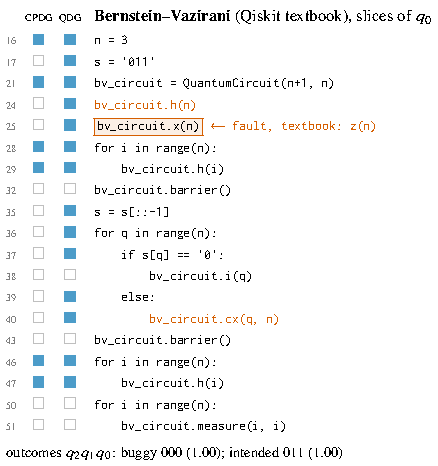
\includegraphics[width=\columnwidth]{figures/fig_bv.pdf}
  \caption{The Bernstein--Vazirani program of the Qiskit textbook~\cite{qiskittextbook}, with comments and
  blank lines omitted and the textbook's line numbers kept. Line~25 carries a seeded fault, \texttt{x(n)}
  where the textbook applies \texttt{z(n)}. The two columns mark the statements in the backward slice of
  $q_0$ under the classical PDG and under the QDG. The classical PDG misses the orange lines, which are
  dependences of $q_0$. Slices are computed by our tool statically, and outcomes and dependences by the
  study's code.}
  \label{fig:bv}
\end{figure}

The Bernstein--Vazirani algorithm~\cite{bernstein1997qct} finds a hidden bit string $s$ with a single query
to an oracle that computes the parity of $s \wedge x$. Fig.~\ref{fig:bv} shows the program of the Qiskit
textbook~\cite{qiskittextbook}, with $s = 011$. The algorithm rests on phase kickback. Lines~24 and~25
prepare the auxiliary qubit $q_3$ in $\ket{-}$, a superposition of $0$ and $1$ with opposite signs. Each
CNOT of line~40 has the auxiliary as its target, and on $\ket{-}$ it leaves the target unchanged and flips
the phase of its control instead. The Hadamard gates of line~47 turn these phases into the bits of $s$. We
seeded one fault, a one-token change on line~25 that applies $X$ instead of $Z$. The auxiliary is then left
in $\ket{+}$, on which a CNOT acts as the identity, and the program returns \numBvBuggyOut{} instead of
\numBvFixedOut{}.

The developer sees $q_0$ read $0$ where $s$ says $1$, and slices backward from $q_0$ to see which
statements determine it. A classical slicer follows data and control dependence. It reads
\texttt{cx(q, n)}, the controlled-NOT that flips its target when its control is $1$, as the assignment
$q_n \leftarrow q_n \oplus q$, which reads $q$ and writes only the auxiliary. Its slice of $q_0$ keeps the
Hadamard gates of lines~\numBvCpdgLines{} and the statements that compute their qubits, lines
\numBvCpdgClassical{}, as the left column of Fig.~\ref{fig:bv} shows. The slice even appears to be right.
Its \numBvCpdgOps{} operations give $q_0$ the same state as the whole program, with fidelity
\numBvCpdgFidelity{}, where fidelity measures the similarity of two quantum states and is $1$ exactly when
they are equal. Two Hadamard gates on $q_0$ show nothing wrong, and the slice gives the developer no
reason to look at lines~\numBvMissedLines{}, where the fault is.

These lines are nonetheless dependences of $q_0$. Restoring $Z$ on line~25 turns $q_0$ from $\ket{0}$ into
$\ket{1}$, two states with fidelity \numBvFixFidelity{}. A CNOT acts on its control as well as its target.
The QDG, in which every gate reads and writes all its qubits, keeps lines~\numBvQdgLines{}, exactly the
dependences of $q_0$, together with the statements that compute them, among them the oracle's loop and
condition on lines~35 to~39. Its slice contains the fault. Entanglement plays no part here, since $q_0$ is in
a pure state after every operation and so is never entangled with the auxiliary.

Choosing a single qubit as the criterion was enough here, because the fault shows in $q_0$ alone. It is not
always enough. In a real bug from Bugs4Q~\cite{zhao2023bugs4q}, posted on Stack Overflow, a two-qubit
program meant to prepare $(\ket{01}+\ket{10})/\sqrt{2}$ applies \texttt{h(1)} where \texttt{x(1)} was
needed, and returns all four bit strings equally often. Each qubit alone reads $1$ with probability
\numMotPOne{}, in the buggy program and in the intended one alike, and the error lies only in the
correlation between the two. A criterion that names a single qubit, as the classical criterion $(s, V)$
does when $V$ is one qubit, cannot express this failure. The criterion must be the pair $\{q_0, q_1\}$.

The two lessons scale. Reading a gate as an assignment misses influence that flows into a control qubit,
and a one-qubit criterion misses errors in correlations.



\begin{figure*}[t]
  \centering
  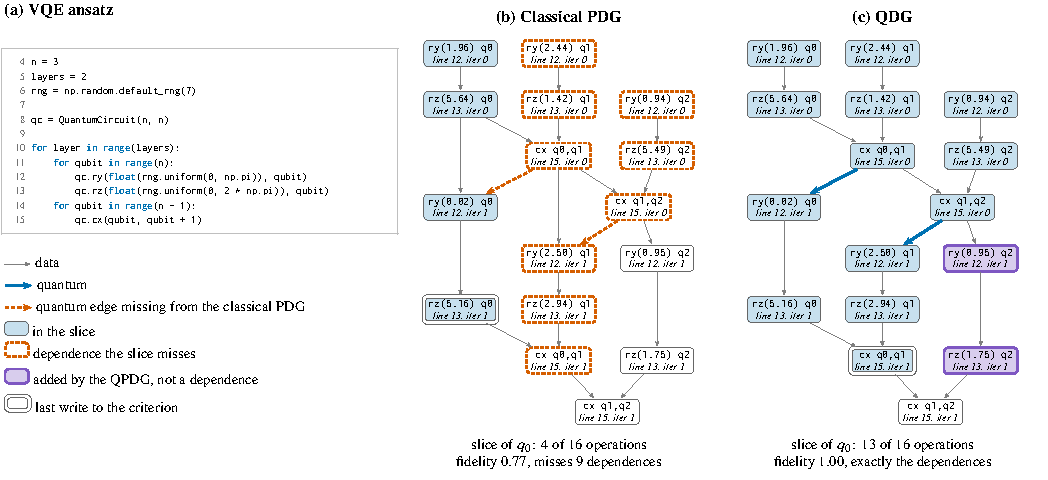
\includegraphics[width=\textwidth]{figures/fig_pdg_ansatz.pdf}
  \caption{Quantum dependence in a variational (VQE) ansatz, criterion $q_0$. Each node is an operation as
  it executes, with the source line and loop iteration that created it, and both graphs place every node at
  the same position. (b)~The classical PDG treats the control of a CNOT as read only. It lacks the orange,
  dashed edges, so its shaded slice of $q_0$ keeps only the rotations of $q_0$ and misses the outlined
  dependences. (c)~The QDG has these edges as quantum edges, and its slice is exactly the dependences
  of $q_0$. The QPDG would also add the purple rotations, which are not dependences. Graphs,
  slices and fidelities at $\ket{0\dots0}$ are computed by the study's code from the program shown.}
  \label{fig:ansatz}
\end{figure*}

\section{Quantum Dependence}\label{sec:dependence}

This section defines what a slice of a quantum circuit must preserve, what an operation's dependence
on a qubit is, and the dependence rules we compare. The definitions are independent of any slicer, and
the evaluation in Section~\ref{sec:results} measures each rule against them.

\subsection{Circuits and their semantics}
A circuit $P = o_0 \dots o_{L-1}$ is a sequence of operations over qubits $Q = \{0, \dots, n-1\}$ and
classical bits $C$. Each operation $o$ acts on a set of \emph{locations} $\mathit{loc}(o) \subseteq
Q \cup C$. A gate acts on its qubits, a measurement on its qubit and the bit it writes, a reset on its
qubit, and a classically conditioned gate on its qubits and the bits its condition reads. For an input
state $\rho$ of the qubits, with every bit initially $0$, $\llbracket P \rrbracket(\rho)$ denotes the
unconditional final state, that is, the joint state of qubits and bits averaged over measurement
outcomes. For $W \subseteq Q$, $\rho_W = \operatorname{Tr}_{Q \setminus W}(\rho)$ is the reduced
state of $W$. For a set of positions $S$, the restriction $P|_S$ keeps the operations at the positions
in $S$, in their original order. Every slicer in this paper returns such a set, and every slice is
judged by running $P|_S$.

\subsection{Criteria, slices, and dependence}

\begin{definition}[Slicing criterion]\label{def:criterion}
A slicing criterion is a nonempty set $W \subseteq Q$ of qubits at the end of the circuit.
\end{definition}

The classical criterion $(s, V)$ names a statement $s$ and variables $V$ used at $s$, and Yu and Zhao
transfer it unchanged to quantum programs~\cite{yu2025qpdg}. A single qubit has no value of its own,
however: its state can be determined only together with the qubits it is correlated with. We therefore
let the criterion be a set of qubits and preserve their \emph{joint} state. $W = \{q\}$ is the
single-qubit criterion.

\begin{definition}[State preservation and soundness]\label{def:sound}
A set of positions $S$ \emph{preserves} $W$ at input $\rho$ if
$\operatorname{Tr}_{Q \setminus W}\llbracket P|_S \rrbracket(\rho) =
\operatorname{Tr}_{Q \setminus W}\llbracket P \rrbracket(\rho)$. $S$ is a \emph{sound} slice for $W$ if
it preserves $W$ at every input.
\end{definition}

Comparing reduced states is basis-independent. It detects phase errors that a measured distribution in
one basis misses. In the experiments, equality means Uhlmann fidelity at least $1 - 10^{-6}$.

Soundness says that the slice reproduces what the criterion qubits end up in. A developer localizing a
fault needs a second guarantee, that the slice contains every place where a fault could change that
outcome.

\begin{definition}[Quantum dependence]\label{def:dep}
Operation $o_k$ is a \emph{dependence} of $W$ in $P$ if there exist an input $\rho$ and a unitary $U$ on
the qubits of $o_k$ such that inserting $U$ immediately after $o_k$ changes
$\operatorname{Tr}_{Q \setminus W}\llbracket P \rrbracket(\rho)$. For a measurement, inverting its
recorded outcome for the conditions that read it also counts as such a change.
$\mathit{Dep}_W(P)$ is the set of dependences of $W$. A set $S$ is \emph{dependence-complete} for $W$ if
$\mathit{Dep}_W(P) \subseteq S$.
\end{definition}

The two properties are distinct. Deleting a single unitary $o_k \notin \mathit{Dep}_W(P)$ leaves
$\rho_W$ unchanged (take $U = o_k^{\dagger}$), but deleting several such operations can change it. A
sound slice, conversely, need not contain every dependence. The ground truth of
Section~\ref{sec:design} approximates the existential quantifiers of Definition~\ref{def:dep} by sampled
inputs and perturbations, so the measured $\mathit{Dep}_W(P)$ is a subset of the true one.

\subsection{Dependence rules}

A \emph{dependence rule} $R$ assigns each operation the locations it reads, $r_R(o)$, and the
locations it writes, $w_R(o)$. Operation $o_j$ depends on $o_i$ under $R$ if $i < j$ and some location
in $w_R(o_i) \cap r_R(o_j)$ is not written by any operation between them. The backward slice
$B_R(W)$ is the set of operations from which the last writer of some $q \in W$ is reachable. A rule can
account for three kinds of dependence. \emph{Data} dependence follows a qubit from the operation that
last changed it. \emph{Control} dependence follows a classical bit from the measurement that wrote it to
the operations its value conditions. \emph{Quantum} dependence lets a multi-qubit gate change every qubit
it acts on, including its controls. We compare three rules that differ in which of these they include,
and two refinements of the most complete one.

\emph{Classical PDG} (CPDG) applies the classical program dependence graph~\cite{ferrante1987pdg} to the
circuit, with data and control dependence. Its data dependence reads a gate as a classical assignment. A
controlled gate reads its controls and targets and writes only its targets, and any other gate reads and
writes all its qubits. Its control dependence follows the classical bits. A measurement writes its bit,
and a conditioned gate reads the bits its condition tests. We also report \emph{def-use} (DU), the same
data dependence without classical bits, as the minimal classical port.

\emph{Wire} (W) adds quantum dependence to the classical PDG. Every operation reads and writes all its
locations, $r_W(o) = w_W(o) = \mathit{loc}(o)$, so a controlled gate also writes its controls. $B_W$ is the
backward light cone of $W$, extended along classical bits from measurements to the gates they condition.

\emph{Entanglement closure} (QPDG) is our documented reading of Yu and Zhao's
graph~\cite{yu2025qpdg}, whose dependences are given informally. It adds to the wire edges an edge from
every operation to every later one when both act on qubits of the same component of the coupling
graph, which links any two qubits joined by a multi-qubit gate anywhere in the circuit.

\emph{Commutation} keeps the operations of $B_W(W)$ that do not commute with the observables
propagated backward from $W$, the union over the Pauli observables $X$, $Y$ and $Z$ on each criterion
qubit, as implemented by Qiskit's \texttt{LightCone} transpiler pass~\cite{javadi2024qiskit}.

\emph{State-based pruning} (QSlice) starts from $B_W(W)$ at a given input, by default $\ket{0\dots0}$.
It removes an operation that does not act on the criterion when the mutual information between the
criterion and the operation's qubits is below $10^{-9}$, and when the removal still preserves $W$ at
that input.

\subsection{Properties}

\begin{theorem}[The wire rule is sound]\label{thm:sound}
For every circuit $P$ and criterion $W$, $B_W(W)$ is a sound slice for $W$.
\end{theorem}

\begin{IEEEproof}
Process $P$ backward with a set of needed locations $N$, initially $W$. Operation $o_k$ joins the slice,
and $N$ grows by $\mathit{loc}(o_k)$, exactly when $\mathit{loc}(o_k) \cap N \neq \emptyset$. This
computes $B_W(W)$. An operation outside the slice acts only on locations outside the current $N$. Such a
trace-preserving operation leaves the reduced state on $N$ unchanged (no-signaling), so removing it
preserves the reduced state of the needed locations at that point, for every input. Induction over
$P$ gives the claim for $W$. The theorem is mechanized in Isabelle/HOL for an abstract model of local
operations whose assumptions are shown satisfiable.
\end{IEEEproof}

\begin{proposition}[The wire rule is dependence-complete]\label{prop:complete}
$\mathit{Dep}_W(P) \subseteq B_W(W)$.
\end{proposition}

\begin{IEEEproof}
Let $o_k \notin B_W(W)$, and let $P'$ insert $U$ after $o_k$. If $U$ were in $B_W(W)$ for $P'$,
then $o_k$, which precedes $U$ on the same locations, would be in $B_W(W)$ for $P$. So $P'$ and $P$
have the same wire slice, and by Theorem~\ref{thm:sound} both preserve $W$. Hence
$\operatorname{Tr}_{Q \setminus W}\llbracket P' \rrbracket(\rho) =
\operatorname{Tr}_{Q \setminus W}\llbracket P|_{B_W(W)} \rrbracket(\rho) =
\operatorname{Tr}_{Q \setminus W}\llbracket P \rrbracket(\rho)$. The argument for an inverted
measurement outcome is the same.
\end{IEEEproof}

The other rules fail one property or the other, as the two programs of Fig.~\ref{fig:dependence} show.
Each node of their graphs is an operation, labelled with the source line that created it, and each edge
is a dependence of the wire rule, marked as data, control or quantum.

Control dependence is needed whenever measurement outcomes steer later gates. In the teleportation
program of Fig.~\ref{fig:dependence}a, the corrections on $q_2$ run only if the measurements of $q_0$
and $q_1$ return $1$. Def-use ignores the classical bits. Its slice of $q_2$ keeps \numTelDuOps{} of the
\numTelOps{} operations, and its fidelity is \numTelDuFidelity{}. The classical PDG follows the control
edges from the measurements to the conditioned gates, and its slice equals the wire slice.

\begin{proposition}[The classical PDG is unsound]\label{prop:du}
There are circuits for which $B_{CPDG}(W)$, and hence $B_{DU}(W)$, does not preserve $W$ even at
$\ket{0\dots0}$.
\end{proposition}

In the ansatz of Fig.~\ref{fig:dependence}c, each \texttt{cx(qubit, qubit + 1)} acts on its control as
well as its target. After the first layer, the state of $q_0$ depends on the rotations of $q_1$ and $q_2$
through these gates. The classical PDG treats a control as read only, so its slice of $q_0$ keeps only
the \numAnsCpdgOps{} rotations on $q_0$ itself, the bold nodes of Fig.~\ref{fig:dependence}d, with
fidelity \numAnsCpdgFidelity{}. The edges it lacks are exactly the quantum edges of the graph. Control
dependence cannot repair this, because the missing dependence is quantum. The wire slice keeps the
\numAnsWireOps{} operations that are dependences of $q_0$, and no other.

\begin{proposition}[Entanglement is neither necessary nor sufficient for dependence]\label{prop:ent}
(i) An operation can be a dependence of $q$ although $q$ is never entangled with its qubits.
(ii) An operation can act on a qubit entangled with $q$ and not be a dependence of $q$.
\end{proposition}

For (i), $q_0$ in the buggy program of Fig.~\ref{fig:motivating} is in a pure state after every
operation, so it is never entangled with anything. Yet \texttt{h(1)} and the CNOT are dependences of
$q_0$, since the fix of line~6 changes the state of $q_0$. For (ii), in
$\mathrm{H}(q_0)\,\mathrm{CX}(q_0, q_1)\,\mathrm{X}(q_1)$ the two qubits are maximally entangled, but
$\mathrm{X}(q_1)$ is not a dependence of $q_0$. No operation on other qubits can change $\rho_{q_0}$
(no-signaling). Entanglement closure therefore adds no dependence that the wire rule misses. It only adds
operations that are not dependences. In Fig.~\ref{fig:dependence}d it adds the \numAnsYzExtra{} rotations
of $q_2$ in the second layer, which run after the last gate that can carry information from $q_2$ to $q_0$.

\begin{proposition}[The wire rule distributes over criteria]\label{prop:joint}
$B_W(W_1 \cup W_2) = B_W(W_1) \cup B_W(W_2)$.
\end{proposition}

\begin{IEEEproof}
By induction over the backward pass of Theorem~\ref{thm:sound}, the needed set for $W_1 \cup W_2$ is
the union of the needed sets for $W_1$ and $W_2$ at every position.
\end{IEEEproof}

Under the wire rule, a joint criterion is therefore the union of single-qubit slices. The criterion
matters for pruning. State-based pruning for $\{q\}$ preserves $\rho_q$ but not the correlations of $q$
with the other qubits, so it can delete an operation that changes $\rho_W$ for a larger $W$. It is also
specific to its input, because the mutual information it tests and the reduced state it checks are
those of one input. Section~\ref{sec:results} measures both effects.

\paragraph*{Superposition}
None of the rules depends on amplitudes. A dependence graph has one node per operation and edges
between operations on shared locations, so superposition cannot enlarge it~\cite{nielsen2010quantum}.
Superposition matters only for state-based pruning, whose checks simulate the circuit and cost time
exponential in its width (Section~\ref{sec:results}).


\begin{figure*}[t]
  \centering
  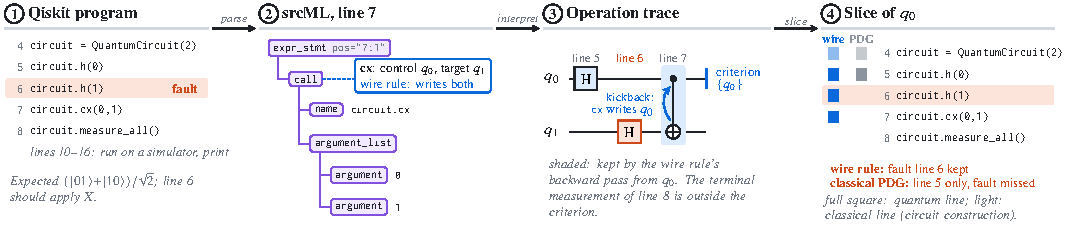
\includegraphics[width=\textwidth]{figures/fig_overview.pdf}
  \caption{The tool slices the Bugs4Q program of Section~\ref{sec:example} statically. srcML parses the
  program in stages 1 and 2, and the letters mark the elements the tool reads. Static interpretation yields
  the operation trace in stage 3, its quantum dependence graph (QDG) in stage 4, and the backward pass from
  the criterion $\{q_0\}$ yields the slice in lines in stage 5. Because \texttt{cx} writes its control $q_0$, the
  faulty line~6 is in the slice. The classical PDG's last writer of $q_0$ is line~5, so it misses the fault.
  The tool computed the figure from the original Bugs4Q file.}
  \label{fig:overview}
\end{figure*}


\section{A Static Slicer for Qiskit Programs}\label{sec:tool}

A slice helps developers only as lines of their program, so we built a tool that slices a Qiskit program
statically with the QDG of Section~\ref{sec:dependence}. Fig.~\ref{fig:tool} shows its steps on the ansatz of
Fig.~\ref{fig:ansatz}.

\paragraph*{Parsing}
The tool parses the program with srcML~\cite{collard2011lightweight, collard2013srcml}, which marks up its
syntax and the position of every element. A table of \numToolGateTable{} Qiskit instruction methods records
which arguments of each are qubits, bits and angles, so that a \texttt{call} element such as
\texttt{qc.cx(qubit, qubit + 1)} becomes a gate on its qubits, as stage~1 of Fig.~\ref{fig:tool} shows.

\paragraph*{Static interpretation}
The tool turns the srcML tree into an operation trace, as Behler et al.\ do for
OpenQASM~\cite{behler2024supporting}. It unrolls loops and records the iteration of each operation, inlines
functions, and follows \texttt{if\_test} and \texttt{c\_if}, Qiskit's constructs for gates conditioned on
measured bits, as stages 2 and 3 of Fig.~\ref{fig:tool} show. Each value carries the lines that computed it,
which gives the classical lines of each operation. Where a
value cannot be resolved statically, the tool over-approximates. An unknown qubit index acts on every qubit
it may denote, an unknown condition runs every branch, and a loop over an unknown range repeats its body
once more than the number of qubits and bits it touches, at most \numToolMaxCopies{} times. Since the needed set never loses a qubit, these over-approximations
only enlarge a slice, and the tool reports each. A circuit passed to code the tool does not model is reported as not traced.

\paragraph*{Slicing}
The slice is the backward pass of Theorem~\ref{thm:sound} on the trace, which skips barriers and terminal
measurements. An operation that may act on several qubits adds all of them to the needed set, and a bit
leaves the needed set only when an operation certainly writes it. The pass returns the operations of the
slice, their lines and iterations, and the classical lines they depend on, in time linear in the trace.

\paragraph*{Forward slices and profiles}
A forward pass over the same trace gives forward slices, dual to the backward ones on our test programs,
and a qubit slice profile combines one pass of each. Over the
\numProfBugsQubits{}, \numProfTextQubits{} and \numProfLintqQubits{} qubits of the Bugs4Q programs, the
textbook and \numProfLintqSample{} sampled LintQ files, the two slices of a qubit differ in length for
\numProfBugsFwdNeBwd{}, \numProfTextFwdNeBwd{} and \numProfLintqFwdNeBwd{} of them.

\paragraph*{Validation}
On \numToolDevPrograms{} runnable programs that we wrote, the static trace equals the circuit Qiskit builds. On \numToolDevSliceEqual{} of them, every slice equals
the circuit-level QDG slice of the study. The remaining program nests conditional blocks, and on
\numToolNestedDraws{} random product inputs the oracle of Section~\ref{sec:design} finds the circuit-level slice
wrong \numToolNestedStudyWrong{} times and the tool's slice never. The tool's line slices equal those of the
study on all \numToolTTwoUnits{} units whose lines the study maps, which include the \numLinesUnits{} units of
Section~\ref{sec:results}. Of the \numToolBugsQiskit{} Qiskit files of Bugs4Q, the \numToolTextbookQiskit{} notebooks of the Qiskit
textbook~\cite{qiskittextbook} and the \numToolLintqQiskit{} programs of LintQ's
corpus~\cite{paltenghi2024lintq}, \numToolBugsCircuit{}, \numToolTextbookCircuit{} and
\numToolLintqCircuit{} yield a circuit, \numToolBugsResolved{} of the Bugs4Q ones without over-approximation.
No Bugs4Q or LintQ program crashes the tool, which takes \numToolBugsMedianMs{}~ms per Bugs4Q program in the median.


\section{Study Design}\label{sec:design}

We ask four research questions.
\textbf{RQ1} asks which dependence definitions give sound and dependence-complete slices.
\textbf{RQ2} asks how much smaller than the wire slice a slice can safely be, and under which inputs the
extra precision holds.
\textbf{RQ3} asks what each definition does to fault localization, by hand, with mutation-based fault
localization and with language models.
\textbf{RQ4} asks what each definition costs in time and memory.

\paragraph*{Pre-registration}
The protocol, including the slicers, metrics, tests, thresholds and the decision rules for the
paper's framing, was committed before any run. Every later change is recorded as a dated deviation
with its reason, and those made after a result are marked as such. The changes that affect this paper
add baselines. The full classical PDG and an order-preserving mapping for Qiskit's \texttt{LightCone}
pass were added after the first runs, and both are reported beside the pre-registered results. No
result enforces an expected outcome. The replication package contains the protocol, the deviations,
the logs of every run, and the commit each run used.

\paragraph*{Circuits}
Corpus~A has \numNCircuits{} circuits of at most \numMaxQubits{} qubits from three benchmark suites,
MQT~Bench (\numCircuitsMqt{} circuits)~\cite{quetschlich2023mqt}, QASMBench
(\numCircuitsQasm{})~\cite{li2023qasmbench} and VeriQBench (\numCircuitsVeriq{})~\cite{chen2022veriqbench}.
Every qubit of every circuit is a criterion, which gives \numNPairs{} circuit--qubit pairs, of which
\numNDynamicPairs{} are in circuits with mid-circuit measurement, reset or classical feedback. We also
generate \numFamCircuits{} circuits with known structure. They cover depth sweeps at fixed width,
multipartite states that are partly uncomputed, chains that entangle, disentangle and re-entangle,
indirect entanglement through a third qubit, and inverse pairs $U \dots U^{\dagger}$. For scale,
corpus~L has \numCorpusLCircuits{} larger circuits of 15 to 20 qubits.

\paragraph*{Oracle and ground truth}
All slices are judged by one independent oracle. It simulates the circuit's unconditional state exactly,
by branching over measurement outcomes, and shares no code with any slicer. It agrees with Qiskit's
statevector simulation to within \numOracleErr{} on random circuits. A slice preserves the criterion when
the Uhlmann fidelity of the criterion's reduced state is at least $1 - 10^{-6}$. The dependences of
Definition~\ref{def:dep} are measured by inserting \numInfluencePerturbations{} random unitaries after
every operation and comparing the criterion's state at \numInfluenceInputs{} inputs, $\ket{0\dots0}$ and
ten random product states. A dependence catalogue of \numCatEntries{} hand-derived cases, including the
examples of Section~\ref{sec:dependence}, checks the ground truth and every slicer before the runs.

\paragraph*{Slicers}
Each rule of Section~\ref{sec:dependence} has an implementation. The classical PDG and def-use
implement their read and write rules directly. The wire rule is a backward slice over per-qubit data edges
and measurement-to-condition edges. Entanglement closure adds the coupling-component edges of our
documented reading of Yu and Zhao's graph~\cite{yu2025qpdg}, with every interpretation choice logged
before the runs. Commutation uses Qiskit's \texttt{LightCone} pass, and state-based pruning uses the
algorithm and thresholds of Section~\ref{sec:dependence}. A variant of state-based pruning takes a set of
qubits as its criterion.

\paragraph*{Robustness}
A slice computed at $\ket{0\dots0}$ is checked again, with its positions fixed, under
\numRobDraws{} random computational-basis inputs, \numRobDraws{} random product inputs and, for circuits
with rotation angles, \numRobDraws{} random rebindings of every angle. A pair is robust if the slice
preserves the criterion in every draw.

\paragraph*{Faults}
We seed faults with \numMutOperators{} operators taken from Muskit~\cite{mendiluze2021muskit},
QMutPy~\cite{fortunato2022qmutpy} and the fault model of García de la Barrera et
al.~\cite{garcia2022testing}. They insert, delete and replace gates, insert and delete mid-circuit
measurements, swap a control with a target, remove a control, re-target an operand, corrupt the
preparation of an entangling gate, and perturb an angle. Of the \numMutants{} mutants,
\numMutantsKilled{} change the measured distribution of at least one qubit. Each such qubit is a unit,
which gives \numRqThreeUnits{} units whose criterion is a qubit the developer would see is wrong. A further
\numMutantsInjured{} mutants change only a qubit's phase and form \numRqThreeSecondary{} secondary units.
For each unit we record whether the slice of the faulty circuit contains the fault site and how many
instructions it keeps. The real bugs come from Bugs4Q~\cite{zhao2023bugs4q}. Of \numBugsFourQTriaged{}
entries, \numBugsFourQIncluded{} are circuit-level faults whose buggy and fixed programs can be ported
mechanically to the current Qiskit. Of these, \numBugsFourQKilled{} change a qubit's measured
distribution, \numBugsFourQInjured{} changes only a phase, \numBugsFourQAlive{} changes no qubit, and
\numBugsFourQExcluded{} exceed the oracle. We map their slices back to the lines of the original Qiskit
programs.

\paragraph*{Fault localization}
Mutation-based fault localization ranks instructions with the Ochiai formula, as for quantum programs
in Ishimoto et al.~\cite{ishimoto2025mbfl}, over the whole circuit and within each slice. In the language
model task, a model sees a faulty circuit, or one of its slices, and the wrong qubit, and names up to
three suspect instructions. We score whether the fault site is among them, on \numTTwoItems{} units
sampled across operators, with two Claude models and two open-weight Qwen2.5-Coder models.

\paragraph*{Statistics}
The confirmatory hypotheses H1 to H5 are tested with exact McNemar tests on paired binary outcomes and
Wilcoxon signed-rank tests on paired sizes, with Holm correction across the five. Effect sizes come
first, with bootstrap 95\% confidence intervals (10{,}000 resamples) and Wilson intervals for
proportions. Everything else is descriptive.


\section{Results}\label{sec:results}

\begin{table}[t]
  \centering
  \caption{RQ1: Slices of the \numNPairs{} corpus-A pairs at $\ket{0\dots0}$. Wrong: slices that do not
  preserve the criterion (dynamic: of the \numNDynamicPairs{} pairs with measurement or feedback).
  Recall and precision are against the semantic dependences; size is the mean share of the circuit. Wire adds quantum dependence to the classical PDG; state-based pruning runs at $\ket{0\dots0}$.}
  \label{tab:rq1}
  \footnotesize\setlength{\tabcolsep}{3pt}
  \resizebox{\columnwidth}{!}{%
  \begin{tabular}{@{}l l r r r r r@{}}
    \toprule
    Rule & Dependence & Wrong & Dyn. & Recall & Prec. & Size \\
    \midrule
    Dependences$^{b}$  & semantic              & --                     & --                       & 1.000                 & 1.000                    & \numDepFloor{} \\
    \midrule
    Def-use            & data                  & \numRqOneDuUnsound{}   & \numDuDynamicUnsound{}   & \numRqOneDuRecall{}   & \numRqOneDuPrecision{}   & \numRqOneDuSize{} \\
    Classical PDG      & data, control         & \numCpdgUnsound{}      & \numCpdgDynamicUnsound{} & \numCpdgRecall{}      & \numCpdgPrecision{}      & \numCpdgSize{} \\
    Wire               & + quantum             & \numRqOneLcUnsound{}   & \numLcDynamicUnsound{}   & \numRqOneLcRecall{}   & \numRqOneLcPrecision{}   & \numRqOneLcSize{} \\
    QPDG reading       & wire + entangl.       & \numRqOneYzUnsound{}   & \numYzDynamicUnsound{}   & \numRqOneYzRecall{}   & \numRqOneYzPrecision{}   & \numRqOneYzSize{} \\
    \midrule
    Commutation$^{a}$  & wire, pruned          & \numLcqUnsound{}       & --                       & \numLcqRecall{}       & \numLcqPrecision{}       & \numLcqSize{} \\
    State-based        & wire, pruned          & \numRqOneQUnsound{}    & \numQDynamicUnsound{}    & \numRqOneQRecall{}    & \numRqOneQPrecision{}    & \numRqOneQSize{} \\
    \bottomrule
  \end{tabular}}\\[2pt]
  {\footnotesize $^{a}$\,On the \numLcqApplicable{} pairs where Qiskit's pass applies; it rejects
  circuits that measure, which leaves no dynamic pair. $^{b}$\,The semantic dependences themselves,
  the smallest dependence-complete slice. They are a reference, not a slicer, so they have no
  soundness value.}
\end{table}

\subsection{RQ1: Which definitions give sound and complete slices?}

Table~\ref{tab:rq1} shows that only the rules with quantum dependence are sound. The classical PDG gives a
wrong slice for \numCpdgUnsound{} of the \numNPairs{} pairs (\numCpdgUnsoundPct{}). Its control
dependence matters on circuits with measurement and feedback, where it is wrong on
\numCpdgDynamicUnsound{} pair against \numDuDynamicUnsound{} for def-use, which ignores classical bits. On
the unitary circuits the two rules are identical, and both are wrong on \numCpdgUnitaryUnsound{} pairs.
Of the dependences the classical PDG misses, \numCpdgMissKickback{} reach the criterion only through a
gate on which the criterion qubit is a control, the phase kickback of Proposition~\ref{prop:du}; only
\numCpdgMissFeedback{} reach it through classical feedback. The confirmatory test H1 confirms that
state-based pruning, which starts from the wire slice, is wrong on fewer pairs than def-use
(\numRqOneQUnsound{} against \numRqOneDuUnsound{}, exact McNemar, Holm \numHOnePHolm{}).

The wire rule is sound on every pair and recovers every dependence (recall \numRqOneLcRecall{}), as
Theorem~\ref{thm:sound} and Proposition~\ref{prop:complete} predict. Our reading of the quantum program
dependence graph is sound for the same reason, since its data edges already follow every qubit of a
gate, but its entanglement edges add operations that are not dependences. Its precision falls from
\numRqOneLcPrecision{} to \numRqOneYzPrecision{}, and its slices grow from \numRqOneLcSize{} to
\numRqOneYzSize{} of the circuit. On the \numFamCircuits{} circuits with known structure, no rule with
quantum dependence is ever wrong, while the classical PDG is wrong on \numFamCpdgUnsound{} of their
pairs. The \numCatEntries{} catalogue cases agree with the hand-derived expectations for every rule.

\begin{figure}[t]
  \centering
  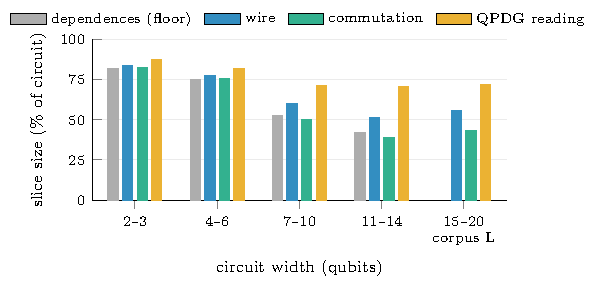
\includegraphics[width=\columnwidth]{figures/fig_size.pdf}
  \caption{RQ1: Mean slice size by circuit width. The grey bars are the dependences, the smallest size a
  dependence-complete slice can have. Corpus~L has no ground truth, which would need exact simulation of
  every perturbation at 15 to 20 qubits. Commutation is shown where Qiskit's pass applies.}
  \label{fig:size}
\end{figure}

Slice sizes should be read against the dependences themselves. The dependences of a qubit make up
\numDepFloor{} of its circuit on average, so no dependence-complete slice can be smaller, and the wire
slice keeps only \numLcExcess{} points more. It equals the dependence set exactly on \numLcExact{} of the
\numNPairs{} pairs, and on \numPairsAllDep{} pairs every operation of the circuit is a dependence. The
QPDG reading keeps \numYzExcess{} points more than the dependences. The sizes are large because most
benchmark circuits are small and densely coupled. Fig.~\ref{fig:size} shows that slices shrink as
circuits widen and less of a circuit can reach one qubit. At 11 to 14 qubits the wire slice keeps
\numWElevenLc{} of the circuit, and on the circuits of corpus~L it keeps \numCorpusLSizeLc{}. The QPDG
reading stays near \numCorpusLSizeYz{}, because entanglement closure links the operations of a whole
coupling component however wide the circuit is. Commutation falls below the floor, to \numWElevenLcq{} at
11 to 14 qubits. It is sound at the tested inputs but not dependence-complete. Deleting a gate that
commutes with the criterion's observables leaves the criterion unchanged, although a different gate at
the same position would change it.

\subsection{RQ2: How much precision beyond the wire slice is safe?}

\begin{figure}[t]
  \centering
  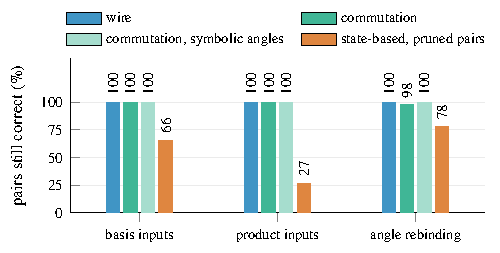
\includegraphics[width=\columnwidth]{figures/fig_robust.pdf}
  \caption{RQ2: Share of pairs whose slice, computed at $\ket{0\dots0}$, stays correct in all
  \numRobDraws{} draws of each input regime. State-based pruning is shown for the
  \numHThreePrunedN{} pairs it prunes; on the others it equals the wire slice.}
  \label{fig:robust}
\end{figure}

Both refinements make slices smaller, but only commutation keeps them correct. State-based pruning
shrinks the wire slice by \numHTwoDiff{} percentage points of the circuit (95\% CI \numHTwoCILow{} to
\numHTwoCIHigh{}), a relative reduction of \numHTwoRelative{}, and is smaller on \numHTwoSmaller{} pairs
(H2, Wilcoxon, Holm \numHTwoPHolm{}). Fig.~\ref{fig:robust} shows what that costs. Of the pairs it
prunes, the slice stays correct for all random product inputs on only \numHThreePrunedRate{}, and over
all pairs on \numHThreeRate{} (Wilson CI \numHThreeCILow{} to \numHThreeCIHigh{}), far below the
pre-registered threshold of 95\% (H3 fails). State-based pruning is therefore a property of one input,
not of the program.

Commutation is smaller than the wire slice on \numLcqSmallerThanLc{} of \numLcqApplicable{} pairs and
stays correct on every random basis and product input. It fails only when the angles change, on
\numRobLcqParamFail{} pairs of variational circuits whose gates commute with the
criterion's observable at their written angle. State-based pruning is only \numQVsLcqReduction{} smaller
than commutation on average, and larger on \numQLargerThanLcq{} pairs. Commutation also misses
dependences (recall \numLcqRecall{}). It drops a gate that commutes with the observable, although a fault
at that gate could still change the criterion.

\subsection{RQ3: What does each definition do to fault localization?}

The wire slice of the faulty circuit contains the fault site in \numRqThreeContainLc{} of the
\numRqThreeUnits{} units, against \numRqThreeContainCpdg{} for the classical PDG,
\numRqThreeContainQ{} for state-based pruning, and \numRqThreeContainRandom{} for a random set of the
state-based slice's size. All \numLcMissTotal{} units the wire slice misses are omission faults, a
removed control (\numLcMissCrm{}), a re-targeted operand (\numLcMissQsw{}), a removed preparation of an
entangling gate (\numLcMissEnt{}) or a deleted gate (\numLcMissDel{}). These faults delete the interaction
that a slice of the faulty program would have to follow, a limit of slicing any faulty program rather
than of the rule.

State-based pruning loses \numHFourLoss{} percentage points of containment against the wire slice
(CI \numHFourCILow{} to \numHFourCIHigh{}), so H4, which allowed a loss of at most five points, fails. In
\numCQFour{} units the wire slice contains the fault and the pruned slice does not. In most of them the
fault makes the criterion separable from qubits it should be correlated with, and pruning then removes the
faulty operation as irrelevant to the single criterion qubit. Slicing with a criterion over all the wrong
qubits recovers \numCQFourRecovered{} of these units. The pruned slices are smaller where both contain the
fault, by \numHFiveSizeDiff{} instructions on average (H5), but the fault then ranks later within them
(EXAM difference \numHFiveExamDiff{}). Mutation-based fault localization confirms that pruning does not
help a ranking. Its mean EXAM score is \numMbflExamAll{} over the whole circuit, \numMbflExamLc{} within
the wire slice and \numMbflExamQ{} within the state-based slice (lower is better).

\begin{figure}[t]
  \centering
  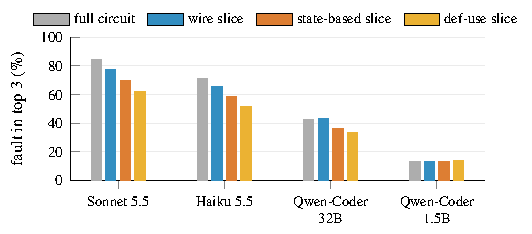
\includegraphics[width=\columnwidth]{figures/fig_llm.pdf}
  \caption{RQ3: Share of the \numTTwoItems{} faulty circuits for which a language model names the faulty
  instruction among its top three, given the whole circuit or a slice of it.}
  \label{fig:llm}
\end{figure}

Language models localize faults worse from pruned slices (Fig.~\ref{fig:llm}). Claude Sonnet~5.5 finds
the fault in its top three for \numTTwoSonnetFull{} of the faulty circuits, \numTTwoSonnetLc{} of the wire
slices and \numTTwoSonnetQ{} of the state-based slices. The state-based slice is
\numTTwoMaxDrop{} points worse than the full circuit (CI \numTTwoSonnetQVsFullCI{}, exact McNemar
\numTTwoSonnetQVsFullP{}) and \numTTwoSonnetQVsLcLoss{} points worse than the wire slice
(\numTTwoSonnetQVsLcP{}). Haiku~5.5 and Qwen2.5-Coder-32B show the same order, and the 1.5B model
localizes too few faults for the input to matter. No slice beats the whole circuit for these models.
Slicing does not hand a model information it lacks; it can only remove the fault.

On the real Bugs4Q programs, the wire slices keep every faulty line, as do the full programs, while
removing little, \numLinesLcMean{} of \numLinesFullMean{} lines on average over \numLinesUnits{} units.
These programs are small. Def-use loses the faulty line in one unit, the bug of
Section~\ref{sec:example}. An independent mapping by the authors' static Qiskit parser agrees with ours
on all \numMapCrossAgree{} instructions both could map.

\subsection{RQ4: What does it cost?}

\begin{figure}[t]
  \centering
  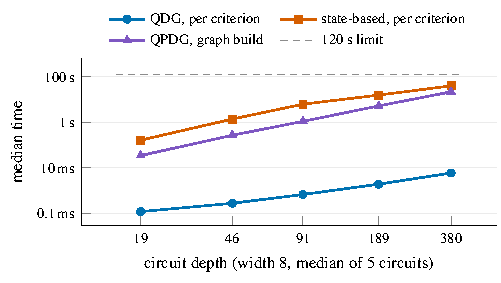
\includegraphics[width=\columnwidth]{figures/fig_cost.pdf}
  \caption{RQ4: Median time per criterion and of building the dependence graph, for circuits of width 8
  and growing depth. At the two largest depths, only the criteria finished within the limit are counted,
  so the state-based time is a lower bound.}
  \label{fig:cost}
\end{figure}

The wire slice costs milliseconds at every depth (Fig.~\ref{fig:cost}), at most \numCostLcMaxMs{}~ms per
circuit. State-based pruning simulates the circuit for every candidate removal. Its time grows with depth
and exceeds the \numCostWallLimit{}~s limit for \numCostDepthEightyOverLimit{} of the 5 circuits at the
second-largest depth and for all \numCostDepthOneSixtyOverLimit{} at the largest. It also grows
exponentially with width, reaching \numCostWidthQMax{}~s at 14 qubits. On corpus~L it completes on
\numCorpusLCompleted{} of \numCorpusLCircuits{} circuits of 15 to 20 qubits. A graph with entanglement
edges is itself costly, because the closure links every pair of operations on a coupling component; the
wire rule needs only the per-qubit edges.


\section{Discussion}\label{sec:discussion}

\paragraph*{Guidance for tool builders}
The results suggest how a slicer for quantum programs should be built. The base should be the wire rule,
in which every gate reads and writes all its qubits. It is sound for every input, misses no dependence,
keeps on average only \numLcExcess{} points more than the dependences, and costs milliseconds. Reading a gate as a classical assignment is the pitfall to avoid, and adding
control dependence does not remove it, since most of the dependences the classical PDG misses are
quantum. Entanglement edges should not be added to make a slice safer. They buy no soundness that the
wire rule lacks and cost precision, because a later operation on an entangled partner cannot change the
criterion's state (Proposition~\ref{prop:ent}). Precision beyond the wire slice can come from
commutation, which stayed correct on every random input but fails when the angles change, so a slicer
for variational programs should recompute it after each parameter update. State-based pruning should be
offered, if at all, as a view of one input, labelled as such, and never as the slice of the program.
Finally, a slicer should let the developer name a set of qubits. Many quantum bugs show only in the
correlation between qubits, as in Section~\ref{sec:example}, and by Proposition~\ref{prop:joint} the
joint wire slice is just the union of the single-qubit slices, so the larger criterion costs nothing
extra.

\paragraph*{Noise and hardware}
A slice is computed statically, so noise cannot change which operations it contains, only whether running
it shows the developer what the full program would. We simulated the pairs of at most ten qubits under
depolarizing noise at three error rates. The noisy state of the criterion under the wire slice differs
from that under the full circuit by at most \numNoiseLcCrossExactMax{} in trace distance where the
simulation is exact, which is rounding error, and by at most \numNoiseLcCrossShotMax{} where mid-circuit
measurements force sampling with \numNoiseShots{} shots. This is what Theorem~\ref{thm:sound} leads one
to expect, since depolarizing noise acts only on the qubits of its gate, so a removed gate and its noise
lie outside the criterion's dependences alike. The state-based slice differs from the full circuit in
\numNoiseQCrossExactNonzero{} of \numNoiseQCrossExactN{} exact runs, by up to \numNoiseQCrossExactMax{}.
It removes noisy gates that the full program executes, and errors accumulate with the number of
gates~\cite{preskill2018nisq}, so it can hide noise the developer is trying to diagnose. On IBM hardware, slices of \numHwCircuits{} circuits from an earlier implementation with
entanglement edges matched the full circuits' measured distributions within a total variation distance of
0.05 for \numHwWithin{}. The other two are QAOA circuits, whose distance is zero in noise-free simulation
and is therefore due to the device, which ran the slice and the full circuit on different physical
qubits. A distance of measured distributions is blind to phase, so these runs show only that slicing
does not break execution on hardware.

\paragraph*{The source level}
A developer reads lines, and a line inside a loop creates one operation per iteration. The line
belongs to the slice when any of them does, so a line-level slice can keep code that no operation-level
slice needs. Fig.~\ref{fig:loops} shows this for the ansatz. In its second layer, the rotations of $q_2$
are not dependences of $q_0$, yet lines 12 and 13 are in the slice. Our tool therefore reports the
iterations of each line. Its static interpretation has limits. A circuit rewritten as a DAG or built
from a QASM string is reported but not traced, and a loop over a range computed at run time is
over-approximated. srcML's markup for OpenQASM~\cite{behler2024supporting, behler2025static} would let
the same back end slice OpenQASM programs.


\section{Related Work}\label{sec:related}

\paragraph*{Program slicing}
Weiser introduced slicing~\cite{weiser1984program} and showed that programmers use slices when they
debug~\cite{weiser1982programmers}. Ottenstein and Ottenstein~\cite{ottenstein1984pdg}, Ferrante et
al.~\cite{ferrante1987pdg} and, across procedures, Horwitz et
al.~\cite{horwitz1990interprocedural} reduced it to reachability in a dependence graph, and dynamic
slicing restricts a slice to one execution~\cite{korel1988dynamic, agrawal1990dynamic}. Surveys cover the
many variants~\cite{tip1994a, harman2008program}. Frameworks such as WALA slice Python through a separate
front end~\cite{wala}, but they see each gate as a call on one circuit object and cannot tell which qubits
an operation depends on. srcSlice computes static slices from the srcML markup of classical
programs~\cite{alomari2014srcslice}, as our tool does for Qiskit programs, but it has no notion of qubits.
A recent retrospective notes that slices can be defined by almost any semantic method and names quantum
programs as a future direction~\cite{gallagher2025program}. Slicing of probabilistic programs preserves
the distribution of the criterion variables~\cite{hur2014slicing, amtoft2020theory, olmedo2025slicing}.
Preserving $\rho_W$ is stronger, since it preserves the outcome distribution of every measurement of $W$,
and a distribution in one basis does not see phase.

\paragraph*{Dependence in quantum programs}
To our knowledge, Yu and Zhao's QPDG~\cite{yu2025qpdg} is the only prior proposal of dependence-based
slicing for quantum programs. Its dependences are defined in prose, and it leaves an implementation and its
evaluation to future work. Its no-cloning example, \texttt{x(0)} followed by \texttt{cx(0,1)}, is described as
entangling the two qubits, although it produces the product state $\ket{11}$, which is case~(i) of
Proposition~\ref{prop:ent}. The quantum code property graph of Kaul et al.~\cite{kaul2023uniform} adds a
data-flow edge from the control of a CNOT to its target and treats the control as unchanged, the classical
reading that Proposition~\ref{prop:du} refutes. LintQ~\cite{paltenghi2024lintq} orders two operations
exactly when they act on a common qubit, the relation of the QDG, to find bug patterns, aiming by design
at neither full soundness nor full precision. Behler et al.\ extend srcML to OpenQASM, analyze the order of
the operations on each qubit~\cite{behler2024supporting}, and name the slicing of individual qubits as
future work~\cite{behler2025static}.

\paragraph*{Entanglement analysis and light cones}
Static entanglement analyses use type systems~\cite{perdrix2007types, prost2009reasoning, yuan2022twist},
abstract interpretation~\cite{perdrix2008entanglement, yu2021abstract}, the stabilizer
formalism~\cite{honda2015stabilizer} or dataflow rules~\cite{xia2025entanglement}, and the ScaffCC
compiler assumes that interacting qubits may be entangled~\cite{javadiabhari2015scaffcc}, the rule of our
QPDG baseline. They answer whether qubits are correlated, and they are not slicers. Heim et al.\ observe
that dependences between quantum instructions should account for commuting
instructions~\cite{heim2020quantum}, and Qiskit's \texttt{LightCone} pass restricts a circuit to the gates
that can reach an observable~\cite{qiskit2025}. Light-cone arguments bound which gates affect an observable
in the analysis of QAOA~\cite{farhi2014qaoa}, and quantum separation logics reason locally about the qubits
a program touches~\cite{zhou2021qsl, le2022qsl}. Theorem~\ref{thm:sound} states the light-cone fact as a
property of slices of a program.

\paragraph*{Debugging quantum programs}
A recent roadmap finds debugging research for quantum programs in an initial phase, with almost no use of
dependence graphs or data-flow analysis~\cite{ramalho2025road}. The slicing it reviews splits a circuit at
breakpoints the developer places~\cite{metwalli2022debugging, metwalli2024testing}, and Qiskit's slicing
utilities partition a circuit by barriers, depth or gate type~\cite{qiskitaddonutils}. Neither has a
criterion. Bug studies~\cite{zhao2021bugpatterns} and Bugs4Q~\cite{zhao2023bugs4q} catalog real faults,
static checkers such as QChecker~\cite{zhao2023qchecker} detect known bug patterns, mutation
tools~\cite{mendiluze2021muskit, fortunato2022qmutpy} and fault models~\cite{garcia2022testing} supply the
faults of our study, and Ishimoto et al.\ adapt mutation-based fault localization to quantum
programs~\cite{ishimoto2025mbfl}. Slicing restricts where these tools look, although RQ3 shows that the
restriction alone does not improve their ranking.


\section{Threats to Validity}\label{sec:threats}

\paragraph*{Construct validity}
We measure dependence by perturbing each operation at \numInfluenceInputs{} inputs, which can miss a
dependence that shows only at other inputs. Rerun with \numGcInputs{} inputs and \numGcPerturbations{}
perturbations, the procedure finds \numGcDepsNew{} dependences
beyond the \numGcDepsBefore{} already measured (\numGcDepsNewPct{}), all inside QDG slices, and no rule's
mean recall moves by more than \numGcRecallShiftQ{}. Missed dependences cannot affect soundness, which is judged by the oracle's
fidelity at a threshold of $1 - 10^{-6}$, far above its error of \numOracleErr{}, and the QDG's soundness
for all inputs is proved. The other rules are judged
at $\ket{0\dots0}$ and on \numRobDraws{} draws per input regime, so they could be wrong at other inputs.
Containing the fault site is a proxy for helping a developer, and we ran no study with developers. The
profile predicates of the LintQ comparison are ours, fixed before the comparison, and show that a profile
exposes a confirmed bug, not that a developer would see it.

\paragraph*{Internal validity}
We recorded every choice of our primary reading of Yu and Zhao's prose before the runs. The reading in which a gate only reads its control, added after the results, is unsound on \numYzRoUnsound{} pairs, so claims
about the QPDG hold for the reading named. Rounding at the $10^{-9}$ thresholds of state-based pruning
flips some decisions on one Bugs4Q program, while \numQRepeatRuns{} fresh runs reproduce all
\numQRepeatPairs{} slices of corpus~A.

\paragraph*{External validity}
Exact simulation limits corpus~A to \numMaxQubits{} qubits, corpus~L reaches
\numCorpusLMaxQubits{} qubits, and Theorem~\ref{thm:sound} covers any width. The circuits come from
benchmarks, and the real bugs are few and small. The rules are stated on circuits and carry over to
other languages, except that a repeat-until-success loop in Q\#~\cite{svore2018qsharp} has no single
circuit and a static slicer must over-approximate its iterations. Seeded faults may differ from
real ones, although \numMutPublished{} of our \numMutOperators{} operators come from published tools and
fault models. Times are measured on one machine, and LintQ's and QChecker's are those their papers report on
theirs, so the comparison of times is indicative. \tool{}'s OpenQASM reader is written in Python and dominates its
time on the largest circuits.


\section{Conclusion}\label{sec:conclusion}

A quantum slice supports comprehension only if it keeps every operation that can change the state of the
qubits the developer asks about. We defined this requirement semantically and measured dependence rules
against it. Reading the control of a gate as unchanged gives wrong slices that look right, entanglement
edges add code that cannot matter, and pruning at one input gives slices of that input only. The QDG is
sound for every input, dependence-complete and cheap, and our srcML-based slicer shows it on Qiskit source
as the lines, iterations and qubit profiles a developer reads.

\section*{Data Availability}
The replication package at \url{https://anonymous.4open.science/r/qslice-replication-5B21} contains the
protocol, the Isabelle/HOL theory, the slicer, the circuits, the run logs and the scripts that regenerate
every number and figure, which its \texttt{reproduce.sh} checks. Seeds and package versions (Python~3.12.2,
Qiskit~2.3.0) are fixed, and the package will be archived with a DOI on acceptance.

\section*{Acknowledgment}
A large language model assisted with drafting the text and the analysis scripts. The authors verified all
content and take full responsibility for it.


\bibliographystyle{IEEEtran}
\bibliography{references}

\end{document}
